\ylDisplay{Akvaarium} % Ülesande nimi
{Tundmatu autor} % Autor
{lahtine} % Voor
{2005} % Aasta
{G 10} % Ülesande nr.
{9} % Raskustase
{
% Teema: Geomeetriline-optika
\ifStatement
Leidke maksimaalne suurendus $k$, mille tekitab sfääriline akvaarium, kui vaadata väljastpoolt selles ujuvat kala. Suurenduse all mõistame siin kala kujutise ja tegeliku kala suuruste suhet. Vee murdumisnäitaja $n = \num{1,3}$. Väikeste nurkade puhul kehtib ligikaudne võrdus $\sin \alpha \approx \alpha$. 
\fi


\ifHint
Sfäärilist akvaariumit saab vaadelda kui õhukest tasakumerat läätse, mis on surutud tasase küljega vastu sirgeseinalist akvaariumi. Lisaks peab arvestama, et läätses lõplikku kujutist tekitav kala ei vasta tegelikule kala asukohale vaid akvaariumis murdumise tõttu asuvale kujutisele, mis on tegelikust kala asukohast $n$ korda lähemal.
\fi


\ifSolution
\begin{center}
	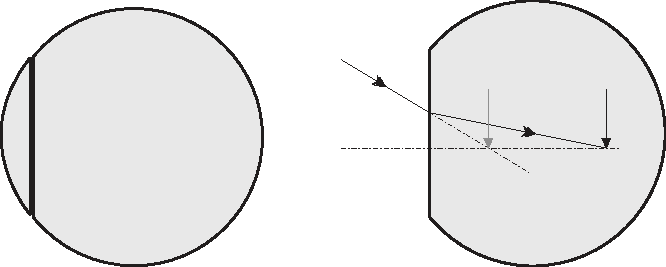
\includegraphics[width=\linewidth]{2005-lahg-10-lah1}
\end{center}

\begin{center}
	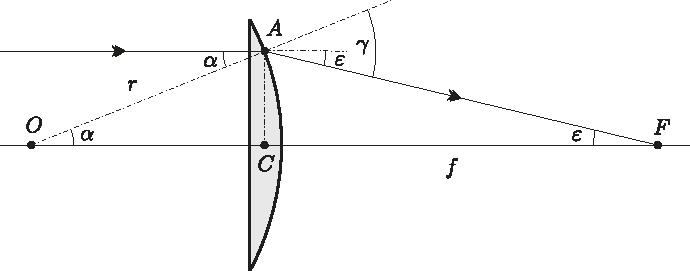
\includegraphics[width=\linewidth]{2005-lahg-10-lah2}
\end{center}

Vaatleme sfäärilist akvaariumi kui õhukest tasakumerat läätse, mis on surutud tasase küljega vastu sirgeseinalist akvaariumi (vt jooniseid). Kasutades väikeste nurkade lähendust on lihtne leida sellise õhukese läätse fookuskauguse $f$ ($f = |CF|$):
\[
\gamma=\alpha n, \quad \varepsilon f=(\gamma-\alpha) f=\alpha r \quad \Rightarrow \quad f=\frac{r}{n-1}.
\]
Vee puhul
\[
f=\frac{r}{\num{1,3}-\num{1}} \approx \num{3,3} r.
\]
Läätses näeme kala kujutist, mis tekib murdumisel akvaariumivees. See kujutis on $n$ korda lähemal akvaariumi seinale, kui kala ise, st maksimaalne kaugus on
\[
l_{\max }=\frac{2 r}{n} \approx \num{1,5} r,
\]
mis on igal juhul väiksem, kui läätse fookuskaugus. Lääts tekitab sellest kujutisest omakorda kujutise, mille kauguse (läätsest) $x$ saame läätse valemist
\[
\frac{1}{f}=\frac{1}{l}-\frac{1}{x}.
\]
On lihtne näha, et suurendus on kahe kujutise kauguste suhe:
\[
\frac{1}{k}=\frac{l}{x}=1-\frac{l}{f},
\]
seega suurendus on maksimaalne, kui $l$ on maksimaalne:
\[
\frac{1}{k_{\max }}=1-\frac{2(n-1)}{n}=\frac{2-n}{n} \quad\Rightarrow\quad k_{\max }=\frac{n}{2-n} \approx \num{1,86}.
\]
\fi
}